\clearpage
\section{Anhang}

\begin{appendix}

\section{Graphen und Fits der Leiterschleife}

\begin{figure}[H]
	\centering 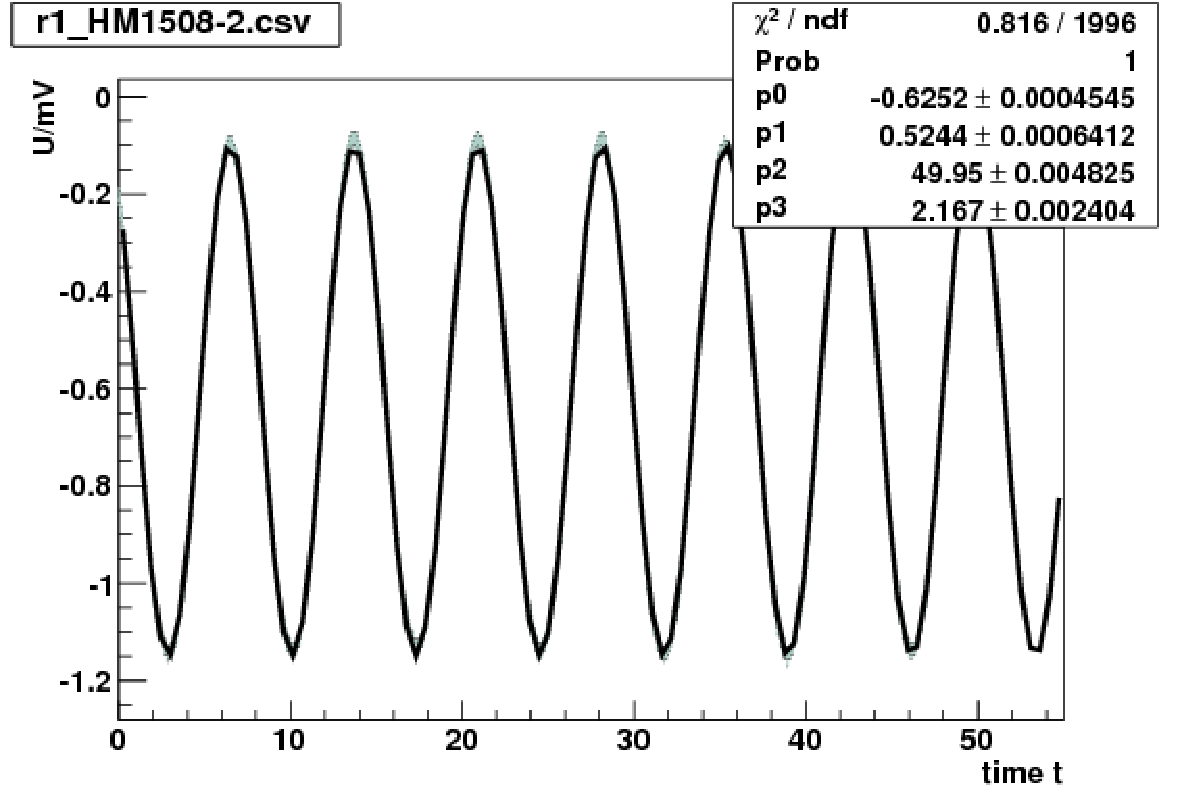
\includegraphics[width=0.9\textwidth]{Auswertung/Widerstaende/r1.pdf}
	\caption{$R_1$}
\end{figure}

\begin{figure}[H]
	\centering 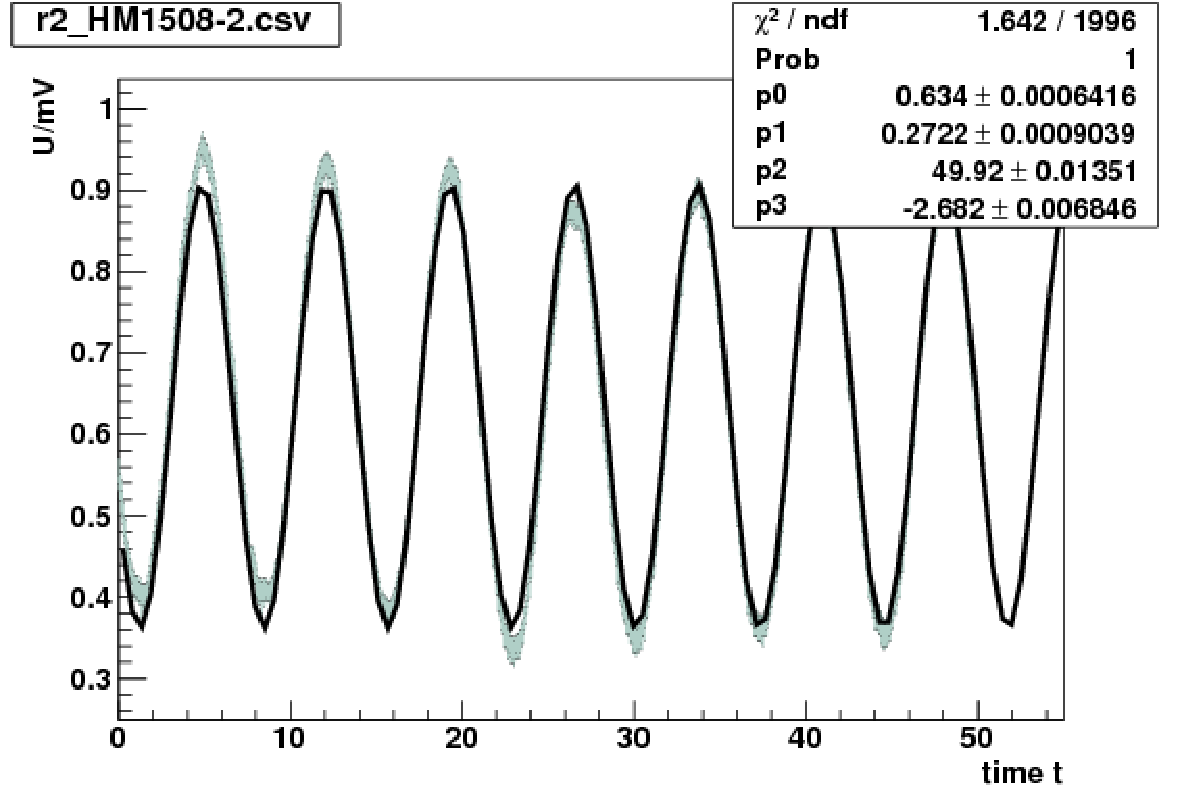
\includegraphics[width=0.9\textwidth]{Auswertung/Widerstaende/r2.pdf}
	\caption{$R_2$}
\end{figure}

\begin{figure}[H]
	\centering 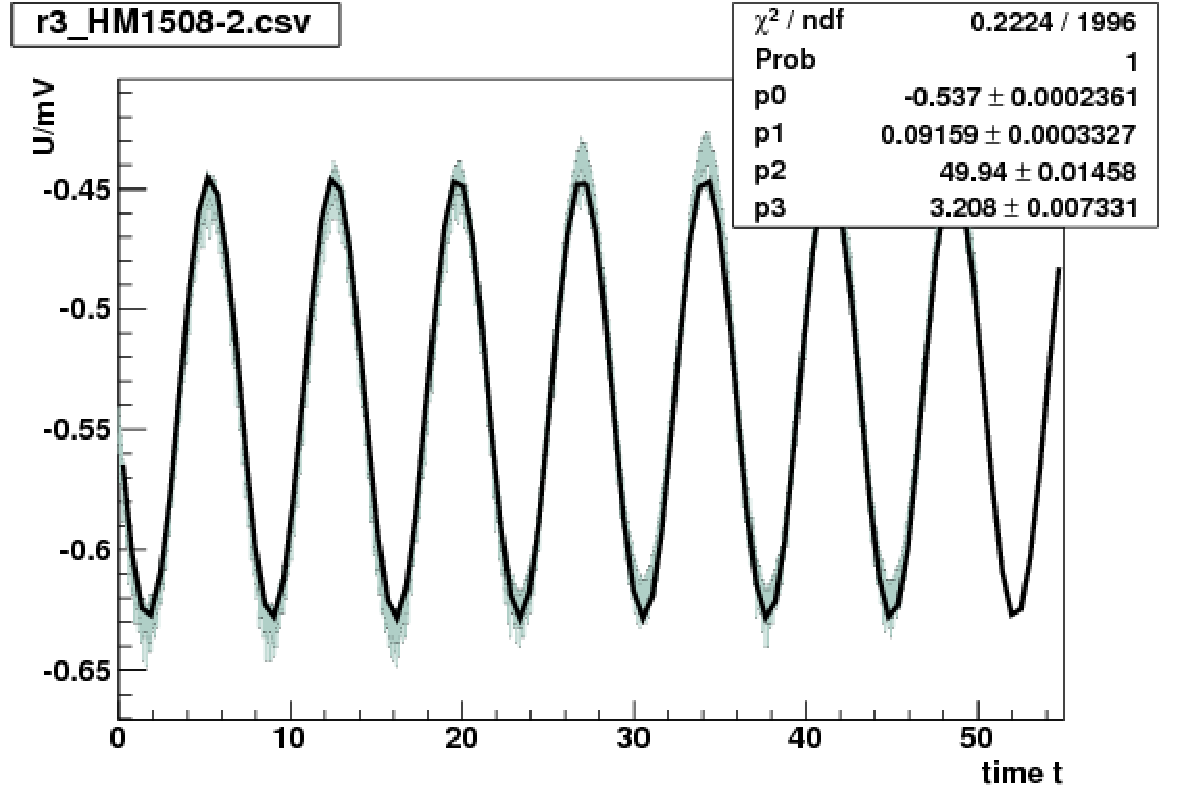
\includegraphics[width=0.9\textwidth]{Auswertung/Widerstaende/r3.pdf}
	\caption{$R_3$}
\end{figure}

\begin{figure}[H]
	\centering 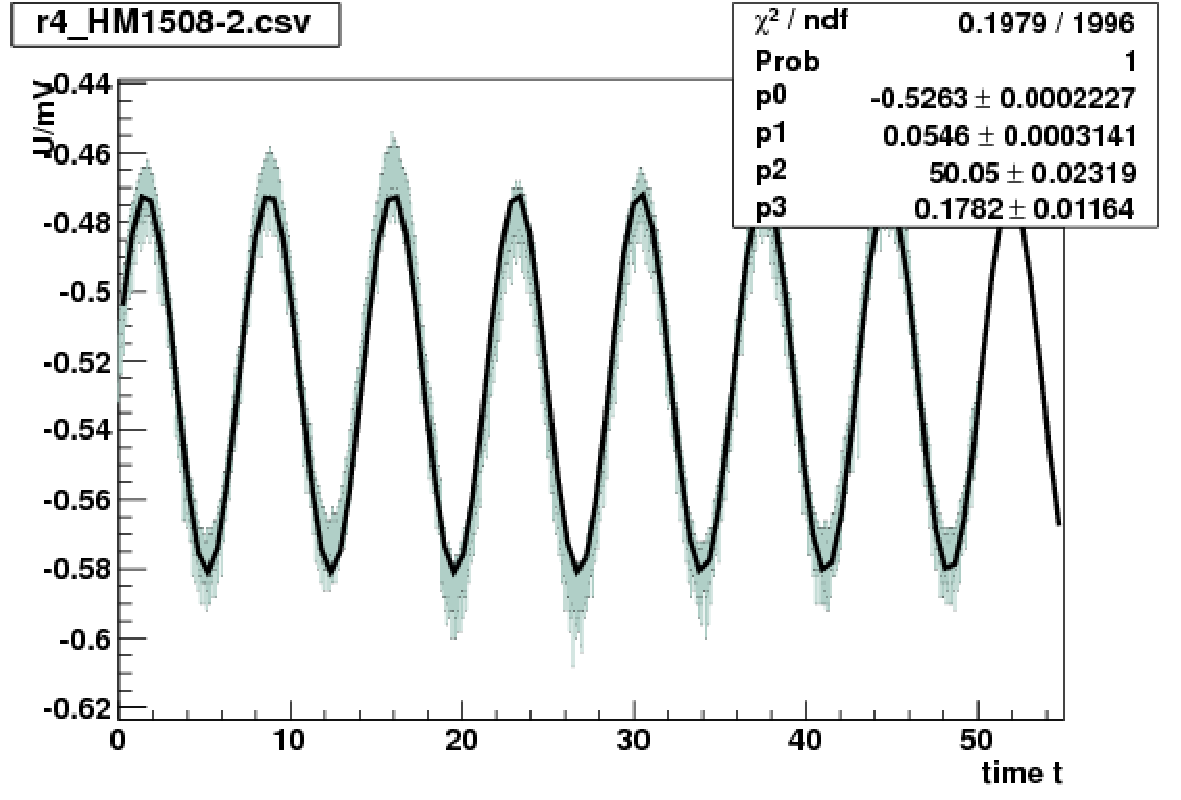
\includegraphics[width=0.9\textwidth]{Auswertung/Widerstaende/r4.pdf}
	\caption{$R_4$}
\end{figure}

\begin{figure}[H]
	\centering 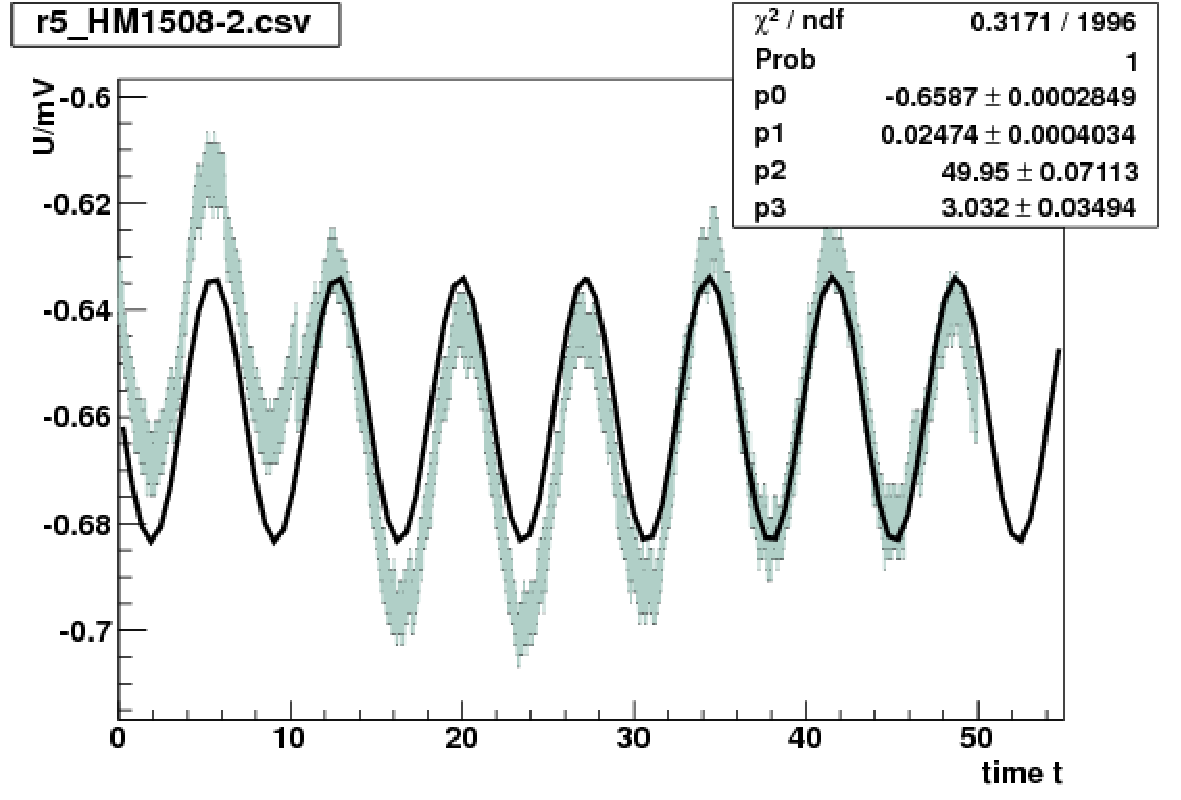
\includegraphics[width=0.9\textwidth]{Auswertung/Widerstaende/r5.pdf}
	\caption{$R_5$}
\end{figure}

\section{Polarplots der Leiterschleife}

\begin{figure}[H]
	\centering 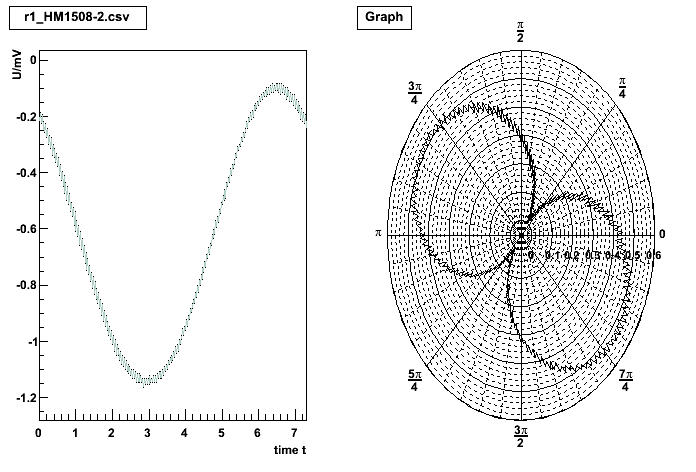
\includegraphics[width=0.9\textwidth]{Auswertung/widerstaende-polar/r1.png}
	\caption{$R_1$}
\end{figure}

\begin{figure}[H]
	\centering 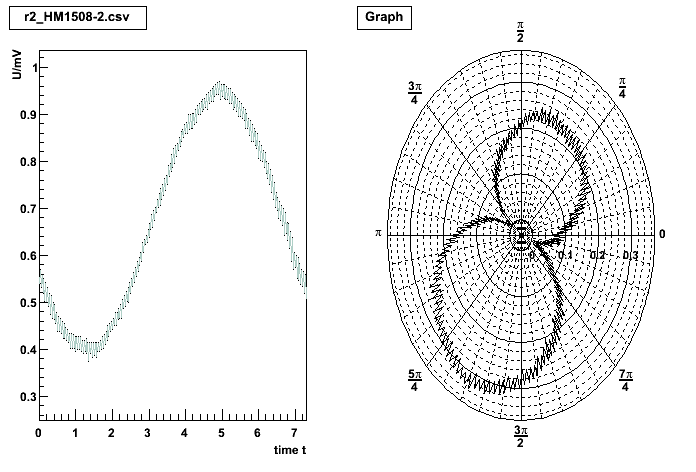
\includegraphics[width=0.9\textwidth]{Auswertung/widerstaende-polar/r2.png}
	\caption{$R_2$}
\end{figure}

\begin{figure}[H]
	\centering 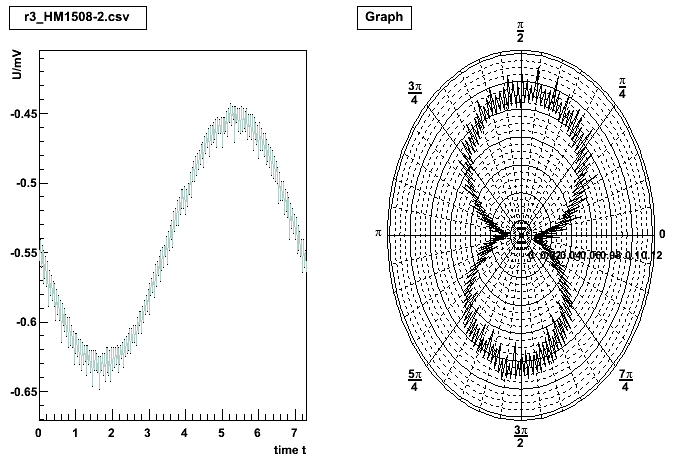
\includegraphics[width=0.9\textwidth]{Auswertung/widerstaende-polar/r3.png}
	\caption{$R_3$}
\end{figure}

\begin{figure}[H]
	\centering 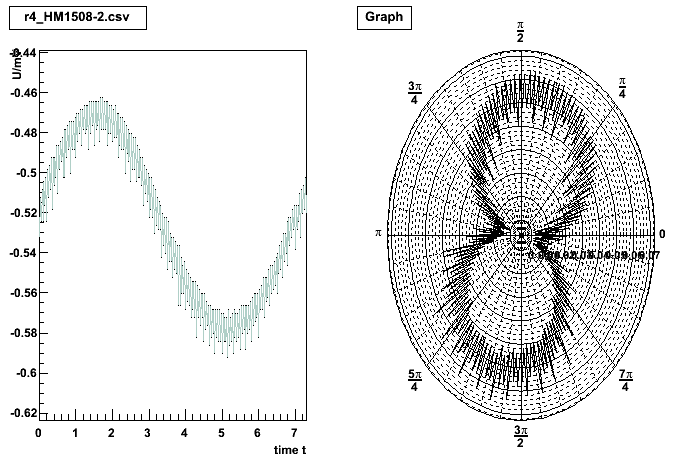
\includegraphics[width=0.9\textwidth]{Auswertung/widerstaende-polar/r4.png}
	\caption{$R_4$}
\end{figure}

\begin{figure}[H]
	\centering 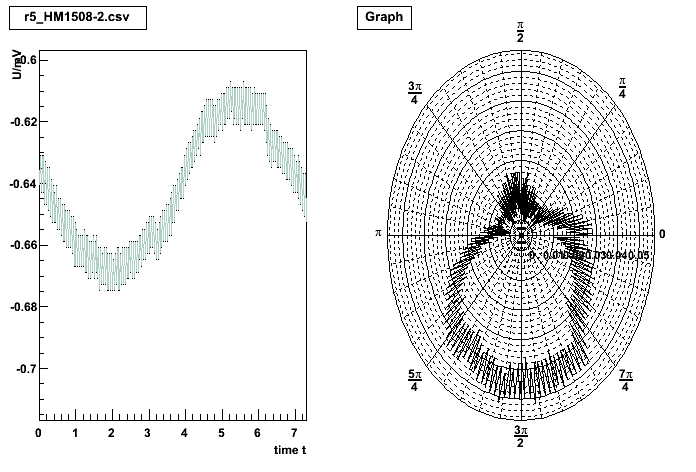
\includegraphics[width=0.9\textwidth]{Auswertung/widerstaende-polar/r5.png}
	\caption{$R_5$}
\end{figure}


\section{Polarplots der Proben}

\begin{figure}[H]
	\centering 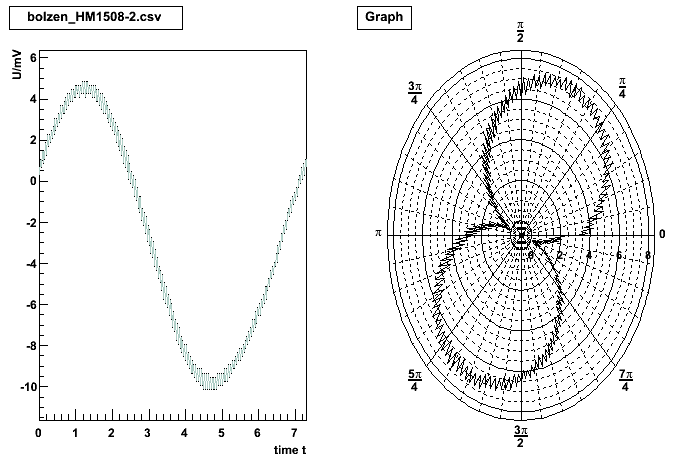
\includegraphics[width=0.9\textwidth]{Auswertung/Proben-polar/bolzen.png}
	\caption{Metallbolzen}
\end{figure}

\begin{figure}[H]
	\centering 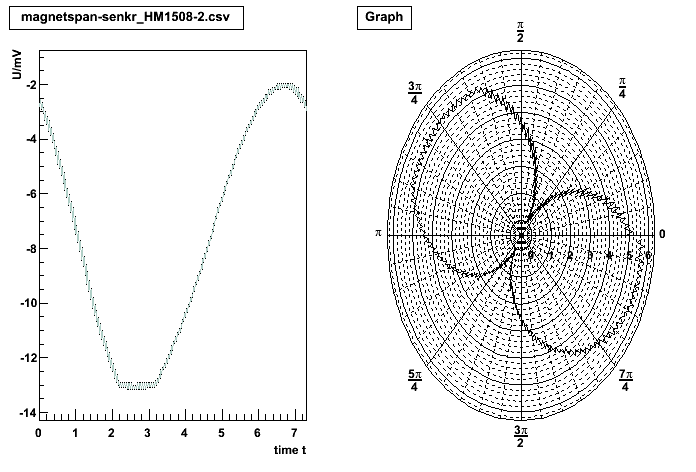
\includegraphics[width=0.9\textwidth]{Auswertung/Proben-polar/magnetspan-senkr.png}
	\caption{Magnetspan $\perp$}
\end{figure}

\begin{figure}[H]
	\centering 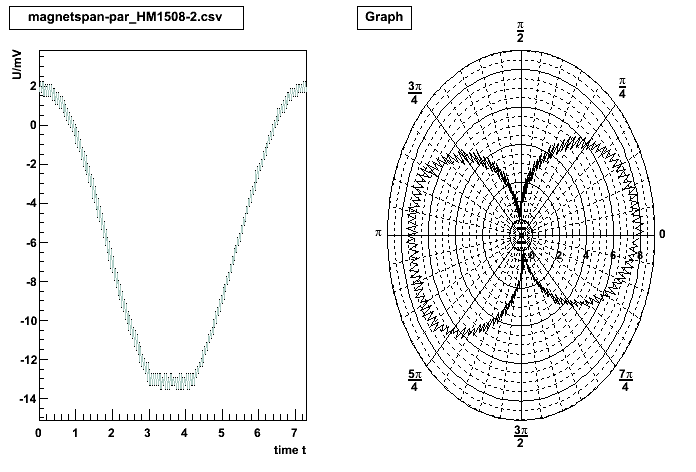
\includegraphics[width=0.9\textwidth]{Auswertung/Proben-polar/magnetspan-par.png}
	\caption{Magnetspan //}
\end{figure}

\begin{figure}[H]
	\centering 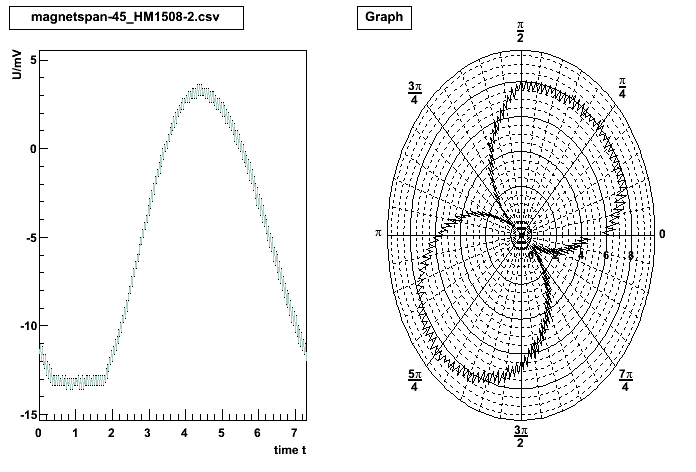
\includegraphics[width=0.9\textwidth]{Auswertung/Proben-polar/magnetspan-45.png}
	\caption{Magnetspan 45$^\circ$}
\end{figure}

\begin{figure}[H]
	\centering 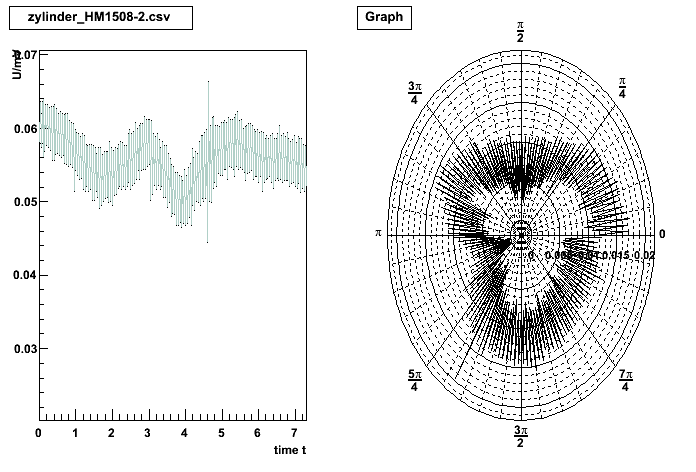
\includegraphics[width=0.9\textwidth]{Auswertung/Proben-polar/zylinder.png}
	\caption{Steinzylinder}
\end{figure}

\begin{figure}[H]
	\centering 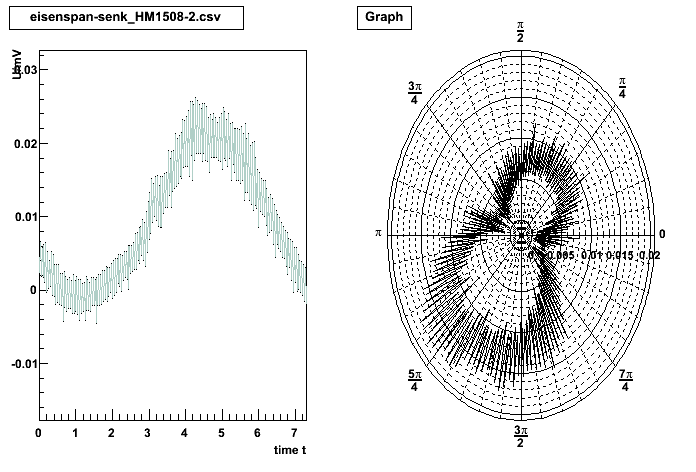
\includegraphics[width=0.9\textwidth]{Auswertung/Proben-polar/eisenspan-senk.png}
	\caption{Eisenspan $\perp$}
\end{figure}

\begin{figure}[H]
	\centering 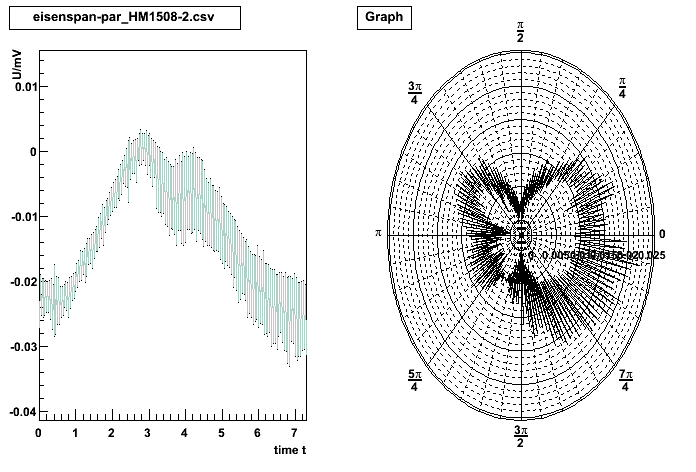
\includegraphics[width=0.9\textwidth]{Auswertung/Proben-polar/eisenspan-par.png}
	\caption{Eisenspan //}
\end{figure}

\begin{figure}[H]
	\centering 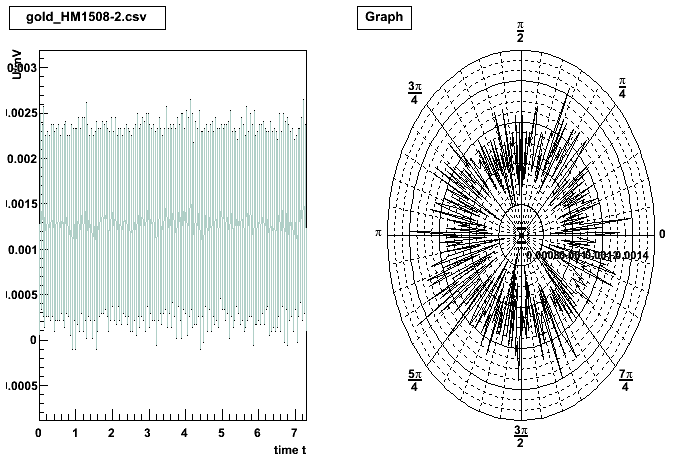
\includegraphics[width=0.9\textwidth]{Auswertung/Proben-polar/gold.png}
	\caption{Gold}
\end{figure}

\begin{figure}[H]
	\centering 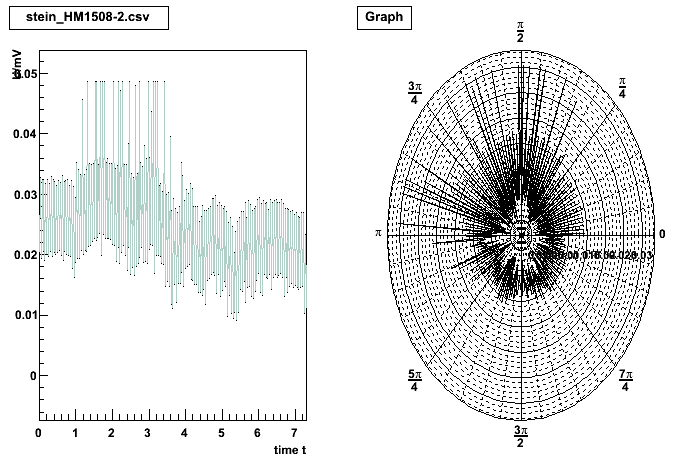
\includegraphics[width=0.9\textwidth]{Auswertung/Proben-polar/stein.png}
	\caption{Heller Kieselstein}
\end{figure}

\begin{figure}[H]
	\centering 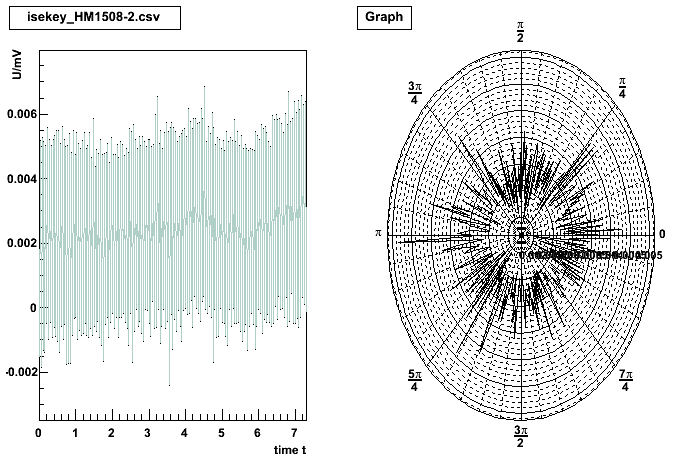
\includegraphics[width=0.9\textwidth]{Auswertung/Proben-polar/isekey.png}
	\caption{Zugangsschlüssel zum ISE}
\end{figure}

\begin{figure}[H]
	\centering 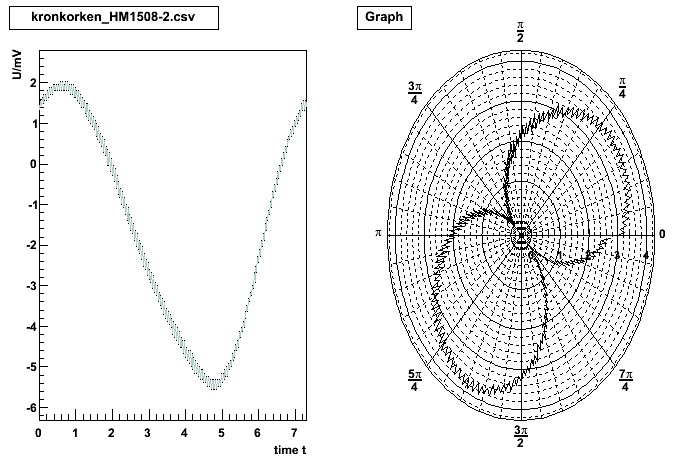
\includegraphics[width=0.9\textwidth]{Auswertung/Proben-polar/kronkorken.png}
	\caption{Kronkorken}
\end{figure}

\begin{figure}[H]
	\centering 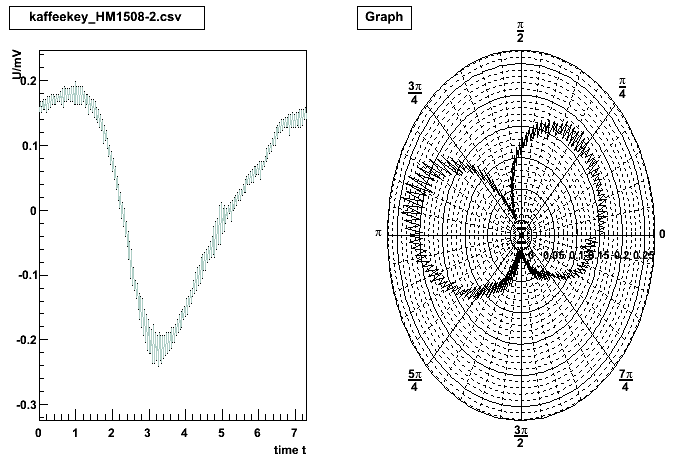
\includegraphics[width=0.9\textwidth]{Auswertung/Proben-polar/kaffeekey.png}
	\caption{Kaffeeschlüssel}
\end{figure}

\begin{figure}[H]
	\centering 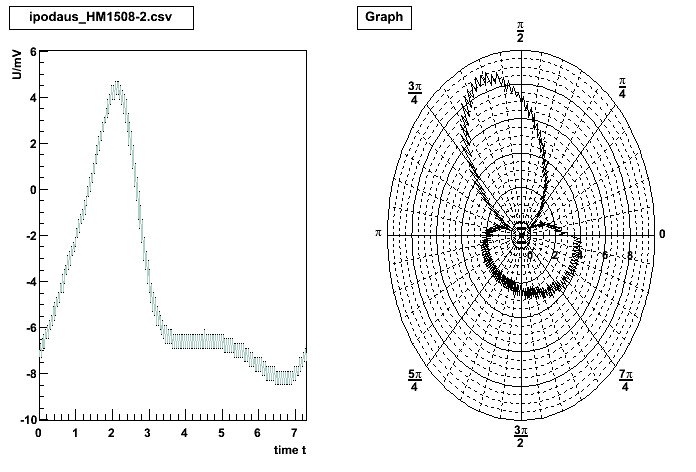
\includegraphics[width=0.9\textwidth]{Auswertung/Proben-polar/ipodaus.png}
	\caption{iPod Shuffle}
\end{figure}


\end{appendix}
